\subsection{Percettrone}
Per comprendere il deep learning occorre prima chiarire il concetto relativo alle reti neurali artificiali (ANN). Il prototipo delle ANN sono le corrispettive biologiche: le reti neurali del cervello umano sono la sede della nostra capacità di comprendere l’ambiente e i suoi mutamenti e di fornire quindi risposte adattive calibrate sulle esigenze che si presentano. Un singolo neurone può ricevere simultaneamente segnali da diverse sinapsi e misurando il potenziale elettrico di tali segnali, stabilisce se è stata raggiunta la soglia di attivazione per generare a sua volta un impulso nervoso. Tale proprietà è implementata anche nelle reti artificiali.

Nel 1958 viene proposta da Rosenblatt la prima rete neurale \textbf{Perceptron}, fatta di un singolo strato con la seguente forma:

\begin{figure}[hbt!]
    \centering
    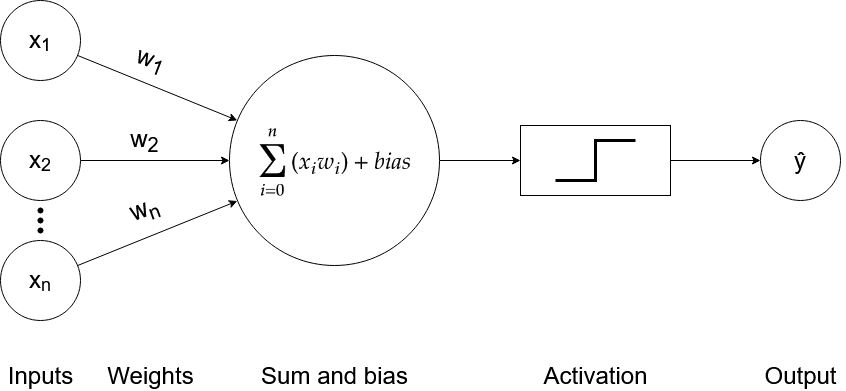
\includegraphics[width=0.9\textwidth]{img/perceptron.png}
    \caption{Percettrone}
    \label{fig:perceptron}
\end{figure}
L'idea di base è di usare diversi pesi per rappresentare l'importanza di ogni input. Se la somma di questi valori è maggiore di un certo valore di soglia, verrà presa una decisione come vero o falso (0 o 1). Nel dettaglio, un percettrone accetta gli input (\(x_1,x_2,...,x_n\)), li modera con dei valori di peso (\(w_1,w_2,...,w_n\)) ed applica loro una funzione di attivazione per produrre il risultato finale. 
La funzione di attivazione, solitamente, è definita come segue:
\begin{equation}
f(x) \ =\ \begin{cases}
        1 & if\ w\cdot x+b > 0\\
        0 & otherwise
    \end{cases}
\end{equation}
Dove:
\begin{itemize}
    \item \textbf{x}: è il vettore degli input
    \item \textbf{w}: è il vettore dei pesi
    \item \textbf{b}: è il bias, una costante che non dipende dai valori in input. Può essere pensato come un livello base di attivazione per l'output.
\end{itemize}

Una volta che abbiamo a disposizione un percettrone, si può cercare di istruirlo in modo che, dato un input \(x\), l'output \(f(x)\) sia quanto più vicino possibile a un dato valore \(g(x)\) scelto a priori.
Guardando la funzione di attivazione, notiamo che, essendo il vettore degli input non prevedibile ed il bias una costante, l'unico valore che è possibile modulare per far si che il percettrone restituisca il risultato desiderato è il vettore dei pesi \(w=(w_1,w_2,...,w_n)\). Infatti, nel cosiddetto \textit{apprendimento supervisionato}, man mano che la macchina elabora output, si procede a correggerla per migliorarne le risposte variando i pesi.

Le capacità computazionali di un singolo percettrone, però, sono limitate e le prestazioni che è possibile ottenere dipendono fortemente sia dalla scelta degli input, che dalla scelta della funzione che si desidera implementare.
